\documentclass[11pt,letter, swedish, english
]{article}
\pdfoutput=1

\usepackage{../../custom_as}
\usepackage[makeroom
]{cancel}
\graphicspath{{figures/}}

\swapcommands{\Omega}{\varOmega}
\swapcommands{\Lambda}{\varLambda}

%%Drar in tabell och figurtexter
\usepackage[margin=10 pt]{caption}
%%För att lägga in 'att göra'-noteringar i texten
\usepackage{todonotes} %\todo{...}

%%För att själv bestämma marginalerna. 
\usepackage[
%            top    = 2.5cm,
%            bottom = 3cm,
%            left   = 3cm, right  = 3cm
]{geometry}

%%För att ändra hur rubrikerna ska formateras
%\renewcommand{\thesubsection}{\arabic{section} (\roman{subsection})}
%\renewcommand{\thesubsection}{\arabic{section} (\alph{subsection})}
%\renewcommand{\thesubsubsection}{\arabic{section} (\alph{subsection},\,\roman{subsubsection})}

%\renewcommand{\thefootnote}{\fnsymbol{footnote}}

\newcommand{\Tc}{\ensuremath{T_{\text{c}}}}
\newcommand{\DE}{\ensuremath{\Delta{E}}}
\newcommand{\sign}{\ensuremath{\text{sign}}}

%\usepackage{tikz}

\begin{document}

%\tikzstyle{every picture}+=[remember picture]
%\tikzstyle{na} = [shape=rectangle,inner sep=0pt,text depth=0pt]



%%%%%%%%%%%%%%%%% vvv Inbyggd titelsida vvv %%%%%%%%%%%%%%%%%

\title{Statistical Physics 2 -- PHYS\,705 \\
Computational project}
\author{Andréas Sundström}
\date{\today}

\maketitle

%%%%%%%%%%%%%%%%% ^^^ Inbyggd titelsida ^^^ %%%%%%%%%%%%%%%%%

\section{The 2D Ising model}

%\subsection{The Ising model}
In this part of the project, we will study the Ising model, which is
governed by the Hamiltonian
\begin{equation}
H=-J\sum_{\ev{i, j}} \sigma_i\sigma_j,
\end{equation}
where $J$ is a coupling constant and the sum is over all nearest
neighbors. 



%\addtocounter{subsection}{-1}
\subsection{The algorithm}
In this part we will Monte Carlo (MC) simulate a 2D Ising model. The
rough outline of the algorithm is:
\begin{enumerate}
\item Initialize a grid, of $L\times L$ lattice points, with values
either $+1$ or $-1$ chosen randomly.
\item Flip one spin and check the change in energy $\DE$.
\begin{itemize}
\item If $\DE\le0$, then keep the new configuration. Record $E$ and
$M$ towards the end mean value for this specific
temperature\footnotemark{}.
\item Else, then the new sate should only be accepted with a
probability of $\exp(-\beta\DE)$. This is done by
\begin{enumerate}
\item Generate a random number $r\in[0, 1]$, and
\item only accept the change if $r<\exp(-\beta\DE)$.
\end{enumerate}
\addtocounter{footnote}{-1}
After this, record the (possibly unchanged) values of $E$ and $M$
towards the mean value for this specific temperature\footnotemark{}. 
\end{itemize}
\item Repeat 2 'til your heart's content.
\end{enumerate}
\footnotetext{\label{ftnt:warm-up}
This should only be done after a certain warm-up period
  from the initialization. For these simulations that warm-up period
  was chosen to be $5\times10^4$ MC steps.}
%\subsubsection{The implementation}
This algorithm was implemented using C (the old one, not ++) as the
programming language. 

\subsubsection{A note on the implementation}
\label{sec:DE}
When we want to get an average of e.g. $E$ over a large number of
iterations, it is much cheaper to make use of the fact that $\DE$ can
be calculated more cheaply. Instead of summing over all sites, we can
just sum over the nearest neighbors to the flipped spin
\begin{equation}
\DE_k = -2J \sum_{i,\,\ev{i,k}}\sigma_k\sigma_i,
\end{equation}
where $k$ is the site that just got flipped. The factor $2$ arises
from the fact that $\sigma_k$ flipped from $\pm1$ to $\mp1$. A similar
methods can be used to calculate $M$. 



%\setcounter{subsection}{0}
%\renewcommand{\thesubsection}{\arabic{section} (\alph{subsection})}
%\renewcommand{\thesubsubsection}{\arabic{section} (\alph{subsection},\,\roman{subsubsection})}
\subsection{MC-step (time) dependence in the energy 
and order parameter}
In this initial part of the computations, we will just look at how the
energy $E$ and order parameter $M$ evolve with the simulation
iterations. This is shown in \figref{fig:EM_all}. We see how the lower
temperature run has much less fluctuations, which we would expect.

We also see in \figref{fig:EM_all} that the system needs a certain
warm-up time before it reaches equilibrium after the
initialization. This warm-up time seems to be just under $10^4$
iterations. So for all the following computations, I've discarded the
first $5\times10^4$ values from each run when calculating different
averages. 



\begin{figure}
\centering
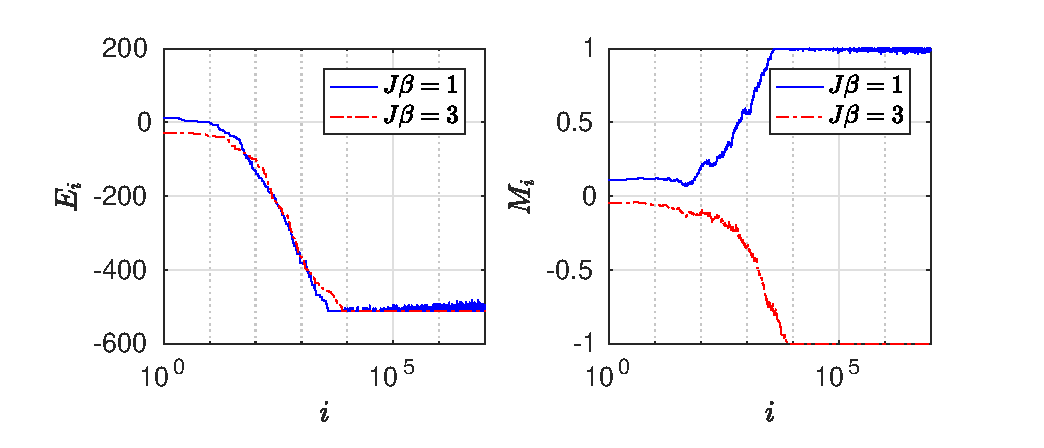
\includegraphics[width=1\textwidth]{EM_all-time-steps.eps}
\caption{Energy $E_i$ and order parameter $M_i$ as a function of
  simulation iteration $i$. Note the log-scale on horizontal axis. We
  see that the lower temperature has much less fluctuation once the
  system has reached an equilibrium. In these cases the equilibrium is
  reached after around $10^4$ iterations.} 
\label{fig:EM_all}
\end{figure}


\subsection{Energy and order parameter as a function of temperature}
From the simulations we can then extract the average energy per spin,
$\ev{E}/N$, and the order parameter, $M$. These are shown in
\figref{fig:EM1}. 

\begin{figure}
\centering
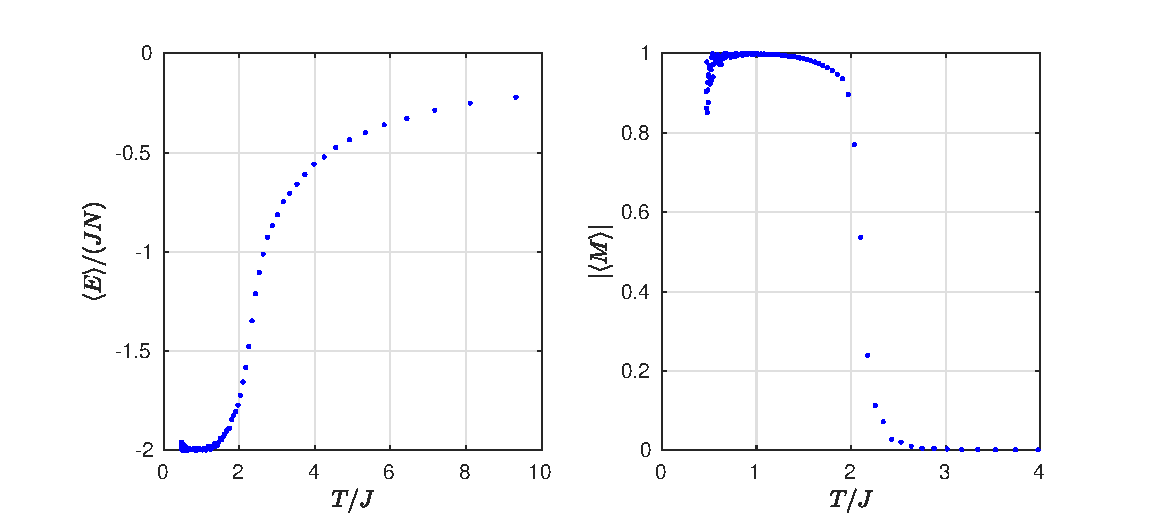
\includegraphics[width=1\textwidth]{EM_L-16_Nsteps-2048_Nmean-16.eps}
\caption{Average energy per spin, $\ev{E}/N$, and order parameter,
  $|\ev{M}|$, in a $16\times16$ grid with periodic BC, as functions of
  $T/J$. The data was produced from a mean of 16 simulations of
  $2\times10^7$ steps each; i.e. each data point for each temperature
  is the average of 16 MC simulations. Note the different temperature
  scales on the two plots.} 
\label{fig:EM1}
\end{figure}


\subsubsection{Averaging over several simulations}
\label{sec:sim_avg}
The simulations were performed according to the algorithm described
above. From the results of the previous section, the first
$5\times10^4$ MC steps were performed \emph{without} recording any
data. Then $2\times10^7$ MC steps were performed, and $E$ and $M$ were
added to the mean values of each parameter.

For the order parameter $M$, which can be both positive and negative with
the same probability, the values in \figref{fig:EM1} are
\begin{equation}\label{eq:evM}
|\ev{M}| = \abs{\frac{1}{N_\text{steps}} \sum_{\text{MC steps}} M}.
\end{equation}
This is not the same as $\ev{|M|}$. The reason for this choice is that
the other one would not become $0$ in the high temperature limit,
since there won't be any negative values in the averaging sum that
could cancel any positive fluctuations. 

Due to unsatisfactory noise levels in the data, first and foremost in
$\ev{M}$ in the transition region with rapid change, the procedure
were performed 16 times over for each temperature. I would argue that
there is a point in taking an average over several simulations, over
just doing a simulation with more time steps. 

That would be because in that transition region with values of
$|\ev{M}|$ in-between 0 and 1, the likelihood of a complete flip in $M$
is higher. I.e. there is a risk of having $M$ hovering around a stable
value $M_0$, but then suddenly flip over to $-M_0$ and staying there
for a while. This risk is obviously greater for $M_0$ closer to $0$,
and with longer simulations. 
A behavior like this will also not be handled well by the averaging
in \eqref{eq:evM}, since changing signs will pull $|\ev{M}|$ towards 0
and not $M_0$. 


\subsubsection{Notes on the behavior of $\ev{E}$ and $\ev{M}$}
The behavior of both $\ev{E}$ and $\ev{M}$, with a rapid change in a
small region at $T$ just over $2J$, suggests that there is a critical
temperature with some phase transitions. But more on this in the next
part. 

We can also note that the asymptotic behavior of the simulated
$\ev{E}$ and $\ev{M}$ seems to correspond to what we would expect
theoretically. 

The order parameter should be $M=0$ above the critical
temperature and below $\Tc$ it should tend towards $\pm1$ as
$T\to0$. We see this behavior in \figref{fig:EM1}, apart from some
``funkiness'' happening at the low end of the temperature spectrum. 

For the energy, we would expect it to go towards 0 in the infinite
temperature limit; we do seem to see that in \figref{fig:EM1}. In the
low temperature limit we would expect all the spins to line up
resulting in an energy of $-2J$ per spin\footnotemark{}, which is also
what we see apart from the same ``funniness'' at the very end of the
temperature range. 
\footnotetext{One could think that we would get $-4J$ per spin as the
  lowest possible energy, due to there being 4 nearest
  neighbors. But then we have to remember that if we just sum up
  all nearest neighbors of every spin site, we would double count all
  ``bonds''; so in the end we have to divide by 2. }

\paragraph{The strange behavior in the lower temperature range}
Before we end this part, we should address the ``funkiness'', in both
$\ev{E}$ and $\ev{M}$, going on in the lower end of the temperature
range. My best guess as to why this happens is because of the random
number generator (RNG) in the standard C library \texttt{stdlib.h}.

That RNG produces an integer value between 0 and about $2\times10^9$
on my computer. That means that the \texttt{double}, that is generated
by diving the random number by the maximum value, will have a
resolution of around $5\times10^{-10}$. 
That random number is then compared to the Boltzmann factor of
$\exp(-\beta\DE)$, which at the lower temperatures can be as small as
$4\times10^{-8}$ -- corresponding to a flip where all spins were
previously aligned, which is most likely the case at low temperatures.  

That would mean that we have a margin of around 2 orders of magnitude.
A slight deviation from a ``true'' uniform RNG could therefore skew the
results on that small of a margin. The study of RNG's is a field of
its own, but I know this much that the basic C RNG is not recommended
to use any more. I, however still used it out of laziness. So this is
my guess as to what might be the reason for the drop in $\ev{M}$ at
the low temperature end of the range. 



\subsection{Using the ``singularity'' of the heat capacity to determine the critical temperature}
Before we can do any data analysis we need a way to calculate the heat
capacity
\begin{equation}\label{eq:CV_start}
C_V = \pdv{\ev{E}}{T} = \pdv{\beta}{T}\pdv{\ev{E}}{\beta} 
= -\frac{1}{T^2}\pdv{\ev{E}}{\beta}.
\end{equation}
To do that we recall from the theory of the 
\emph{Canonical ensemble} that 
\begin{equation}
\ev{E} = \frac{1}{Z}\sum_{\{\sigma\}} H\ee^{-\beta H}
= \frac{1}{Z} \pdv{\beta}\sum_{\{\sigma\}} -\ee^{-\beta H}
= -\frac{1}{Z} \pdv{Z}{\beta}.
\end{equation}
Continuing \eqref{eq:CV_start} with this yields
\begin{equation}
C_V = -\frac{1}{T^2}\pdv{\beta}
\qty[-\frac{1}{Z} \pdv{Z}{\beta}]
=\frac{1}{T^2}\qty[
\frac{1}{Z} \pdv[2]{Z}{\beta}
-\frac{1}{Z^2} \pdv{Z}{\beta}\pdv{Z}{\beta}].
\end{equation}
Clearly the second term in the brackets is $\ev{E}^2$, and the first
term is
\begin{equation}
\frac{1}{Z} \pdv[2]{Z}{\beta}
=\frac{1}{Z} \pdv[2]{\beta}\sum_{\{\sigma\}} \ee^{-\beta H}
=\frac{1}{Z} \sum_{\{\sigma\}} (-H)^2 \ee^{-\beta H}
= \ev{E^2}.
\end{equation}
Therefore
\begin{equation}\label{eq:CV}
C_V = \frac{\ev{E^2}-\ev{E}^2}{T^2}.
\end{equation}


\begin{figure}
\centering
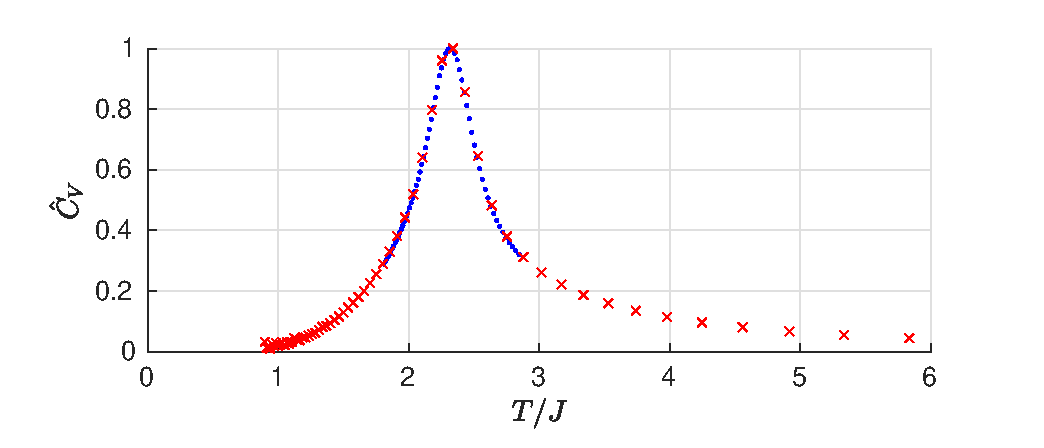
\includegraphics[width=1\textwidth]{CV_L-16_all.eps}
\caption{The heat capacity according to \eqref{eq:CV}, but normalized
  so that the peak would be at 1, in a $16\times16$ grid. We have a
  peak in $C_V$, and it's at around $T=2.32J$.  
  Each data point marked by crosses are the mean of 16 MC simulations,
  while the denser points marked by dots are the means of 128 MC
  simulation. } 
\label{fig:CV1}
\end{figure}


The heat capacity calculated according to \eqref{eq:CV} from a
series of simulation, done in the transitions region of
\figref{fig:EM1}, is shown in \figref{fig:CV1}. There is a clear peak
in the heat capacity, but it's a bit off from the exact 2D Ising
($N\to\infty$) critical temperature of 
$\Tc = 2/\ln(1+\sqrt2) \approx 2.27J$, but not by far. That
discrepancy is probably due to the finite size of the system.


\subsection{Finite size scaling of the susceptibility and critical exponents}
As in the previous part, we need an expression for the susceptibility
\begin{equation}\label{eq:chi_start}
\chi = \eval{\pdv{\ev{M}}{B}}_{B=0}.
\end{equation}
And again we use the theory of the Canonical ensemble to get
\begin{equation}\label{eq:evM}
\ev{M} = \frac{1}{Z}\sum_{\{\sigma\}} \ev{\sigma_i}'\ee^{-\beta H},
\end{equation}
where $\ev{\sigma_i}' = \sum_i\sigma_i/N$ is the
average\footnotemark{} value of all $\sigma_i$'s for each specific
state in $\{\sigma\}$. We also need to modify the Hamiltonian slightly 
\begin{equation}
H = -J\sum_{\ev{i, j}} \sigma_i\sigma_j
-B\sum_{i} \sigma_i
=-BN\ev{\sigma_i}' -J\sum_{\ev{i, j}} \sigma_i\sigma_j.
\end{equation}
Therefore \eqref{eq:evM} can be written as
\begin{equation}
\ev{M} = \frac{1}{Z} 
\pdv{B}\qty[\frac{1}{\beta N}\sum_{\{\sigma\}}\ee^{-\beta H}]
=\frac{1}{\beta N}\,\frac{1}{Z}\pdv{Z}{B}.
\end{equation}
So \eqref{eq:chi_start} can be written as
\begin{equation}
\chi = \frac{1}{\beta N} 
\eval{\pdv{B}\qty[\frac{1}{Z}\pdv{Z}{B}]}_{B=0}
=\frac{1}{\beta N} 
\eval{\qty[\frac{1}{Z}\pdv[2]{Z}{B}
-\frac{1}{Z^2}\qty(\pdv{Z}{B})^2]}_{B=0}.
\end{equation}
And as before, the second term is clearly $(\beta N\ev{M})^2$ while te
first term is
\begin{equation}
\frac{1}{Z}\pdv[2]{Z}{B}
=\frac{1}{Z}\pdv[2]{B}\sum_{\{\sigma\}}\ee^{-\beta H}
=\frac{1}{Z}\sum_{\{\sigma\}}
\qty(\beta N\ev{\sigma_i}')^2\ee^{-\beta H}
=\qty(\beta N)^2\ev{M^2}.
\end{equation}
So
\begin{equation}\label{eq:chi}
\chi =\beta N \qty[\ev{M^2} - \ev{M}^2]
=N \frac{\ev{M^2} - \ev{M}^2}{T}.
\end{equation}
\footnotetext{The prime on the $\ev{\,\cdot\,}'$ is to mark that this is
  not a thermodynamic average.}
We can also note that the modified Hamiltonian won't affect the
behavior in the end, since we're setting $B=0$ after the derivatives.

\figref{fig:chi1} shows the susceptibility calculated as above as a
function of temperature. 


\begin{figure}
\centering
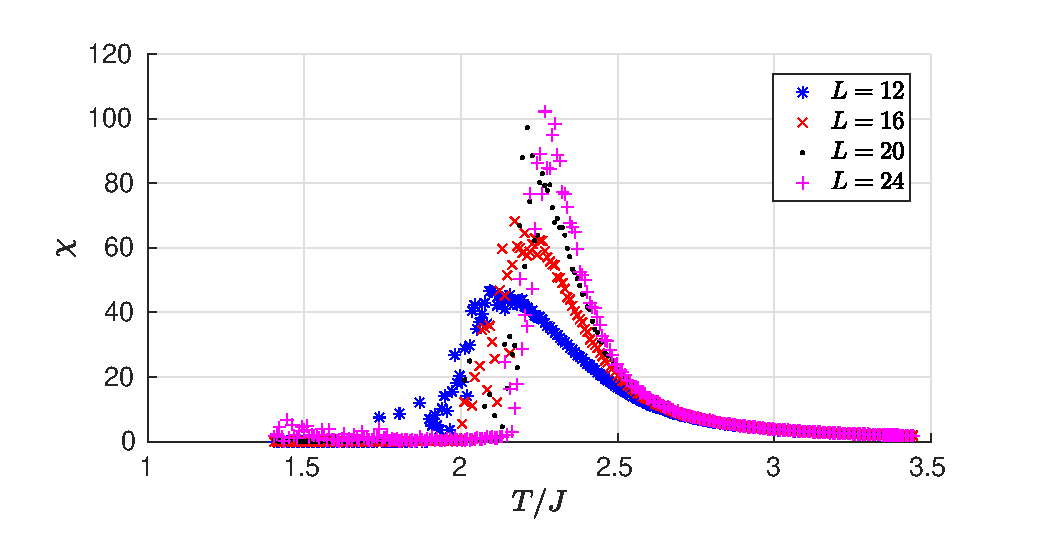
\includegraphics[width=.7\textwidth]{chi_L-16--24_Nsteps-2048_Nmean-16.eps}
\caption{The magnetic susceptibility according to \eqref{eq:chi},
  plotted for 4 different grid sizes. The grids were of size 
  $L\times L$. Each data point is the mean of 8 MC simulations.}
\label{fig:chi1}
\end{figure}

\paragraph{Finite size scaling}
Next we know from class that for a finite size system the scaling
relation for $\chi$ becomes
\begin{equation}
\chi\sim L^{\gamma/\nu}\varPhi\qty(t\,L^{1/\nu}),
\end{equation}
where $L$ is the linear dimension of the system. This means that
plotting $\chi\,L^{-\gamma/\nu}$ against $t\,L^{1/\nu}$, should look
the same independent of $L$. 

This method has been applied to the susceptibilities from above. The
result is shown in \figref{fig:finite-scaling1}. The first thing we
notice with the curves in \figref{fig:finite-scaling1} is that they
don't seem to agree very well in the region $t\,L^{1/\nu}=-2$ to $0$;
that is also by far the noisiest region. But outside of that region we
managed to get a reasonably good collapse onto one single curve. 

The critical exponents were determined by plotting $\chi\,L^{-b}$ 
against $t\,L^{a}$, and then varying $a$ and $b$ independently until
we got a good match. That is in the end the values of $a$ and $b$
relied on visual inspection, which isn't very reliable. By trying to
vary $a$ and $b$ from the optimal values until the curved disagreed
``too much'', we also got a measure on the uncertainty in the critical
exponents. In the end the results were
\begin{equation*}
\nu = 1.1\pm0.1\qcomma\text{and} \quad
\gamma = 1.7\pm0.2.
\end{equation*}
Which isn't too far off from the exact values of $\nu=1$ and
$\gamma=7/4$; the exact values are within the margin of uncertainty,
even though $\nu$ is a borderline case here. 

\begin{figure}
\centering
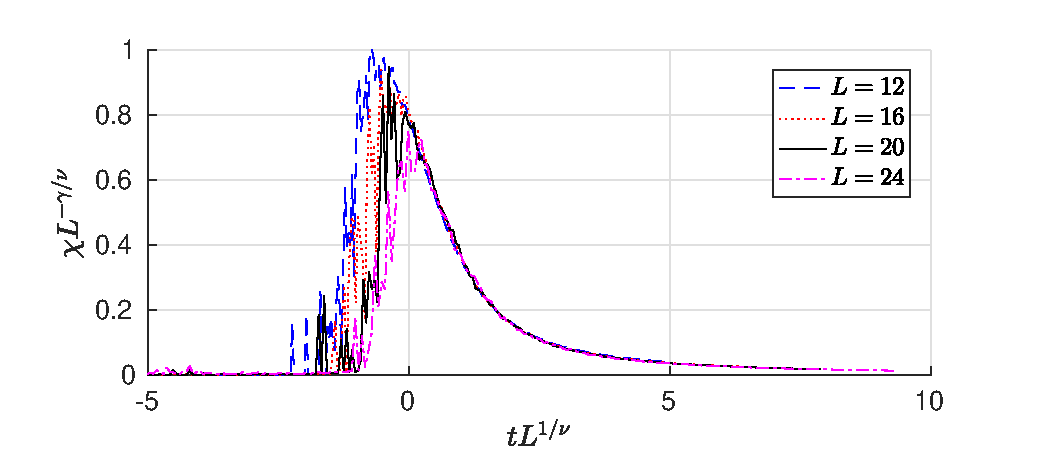
\includegraphics[width=.9\textwidth]{finite-scaling_L-16--24_Nsteps-2048_Nmean-16.eps}
\caption{Finite size scaling applied to the susceptibilities in
  \figref{fig:chi1} with $\nu=1.1$ and $\gamma=1.7$}
\label{fig:finite-scaling1}
\end{figure}

\subsubsection{Error sources}
The most obvious error source here comes from the risk of being
biased when I as a human has to decide which values give a good
fit. Especially when knowing the exact 2D Ising values for the
exponents, it becomes hard to ignore that unconscious bias. The best
solution would be to write some algorithm calculating the internal
discrepancies between the curves and then minimizing that with respect
to $a$ and $b$. But that would require more time than I have for this
project. 

Another topic which needs addressing is what is happening in region
$t\,L^{1/\nu}=-2$ to $0$. Due to the noisiness of the data in that
region, I disregarded the curves there when trying to find a good
fit. 
The noise in that region probably come from similar effects as the one 
described in the end of section~\ref{sec:sim_avg}. This time, averaging
over many simulation runs will not be fully as helpful as before,
because of the non-linearity of the expression for $\chi$.  

Despite the noise however, we do see that that the overall trend
is that the curves do \emph{not} collapse to one there; they are
clearly ordered with $L=12$ being above 16, then 20 and 24 at the
bottom. 
We can see a reason for this discrepancy in \figref{fig:chi1}, where
the peaks of $\chi$ isn't at the same temperature. In the finite size
scaling, we did however just use the exact 2D Ising critical
temperature $\Tc=2/\ln(1+\sqrt2)$ for all sizes. This caused the
curves (primarily $L=12$) to overshoot into the negative regime, which
them made it hard to rescale all of them at once there. This same
effect is probably also causing errors in the values of $\nu$ and
$\gamma$. Maybe we could get better results if we used some kind of
adjusted $\Tc$ for each $L$. 



%%%%%%%%%%%%%%%%%%%%%%%%%%%%%%%%%%%%%%%%%%%%%%%%%%%%%%%%%%%%%%%%%%%%%%
%%%%%%%%%%%%%%%%%%%%%%%%%%%%%%%%%%%%%%%%%%%%%%%%%%%%%%%%%%%%%%%%%%%%%%
%%%%%%%%%%%%%%%%%%%%%%%%%%%%%%%%%%%%%%%%%%%%%%%%%%%%%%%%%%%%%%%%%%%%%%



\section{The XY model}
\newcommand{\rhos}{\rho_{\text{s}}}
\newcommand{\TKT}{T_{\text{KT}}}

In this part we have a Hamiltonian that is
\begin{equation}
H = -J\sum_{\ev{i, j}} \cos(\theta_i - \theta_j).
\end{equation}
The simulations are very similar in nature, where the only change is
that the randomly chosen spin is changed by a random angle instead of
just flipped. Other than that, the main algorithm is just the same as
before. 

\subsection{Some notes on the coding}
For this model, the computations at each time step is more expensive
than for the Ising model, e.g. the spin stiffness
\eqref{eq:rhos} can not be calculated so easily with the same idea
used in section~\ref{sec:DE}. Therefore, to save time I've only
calculated the relevant values at every $N$th iteration, where
$N=L^2$. 
%Arguably this should also be done for the Ising model, but
%the strong correlation between iterations shouldn't affect the
%averages in the end result. 

Another note here is that one has to be careful when calculating the
spin stiffness according to \eqref{eq:rhos}. Especially when
calculating the sum of sines. The thing to keep in mind is the
direction factor, $\vb*r_{ij}\vdot\vu{e}$. With out it you will only
have terms of the form
\begin{equation}
\sin(\theta_k - \theta_l) + \sin(\theta_l - \theta_k) =0
\end{equation}
if you are not careful. 

\subsection{Energy and heat capacity}
Just as before we can study the energy and the heat capacity of the
system. When we do that, we get the result in \figref{fig:ECV2}. And
once again we see a trend in the energy to be dropping for lower
temperature, however not as dramatically as for the Ising model. 
The heat capacity still shows a peak, however the peak is at a
temperature higher than $\TKT$. 

\begin{figure}
\centering
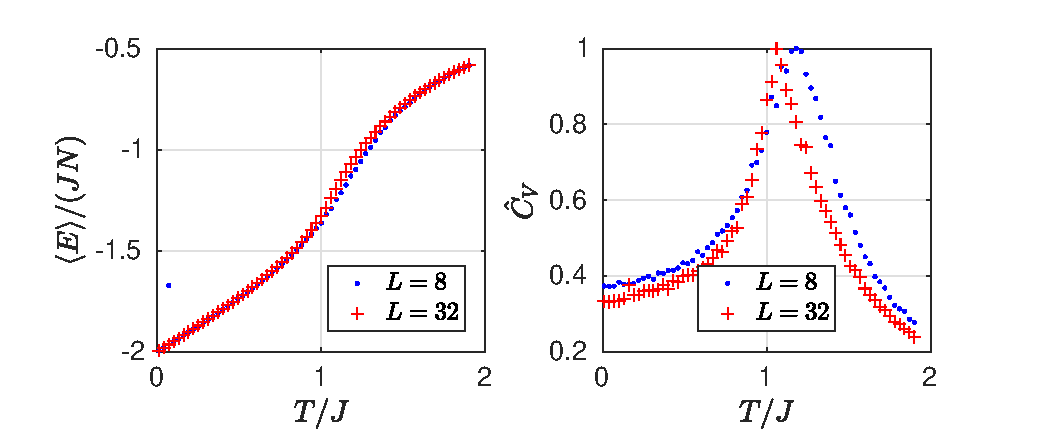
\includegraphics[width=1\textwidth]{XY_ECV_L-8-32_Nsteps-64.eps}
\caption{Average energy per spin, $\ev{E}/N$, and normalized heat
  capacity $C_V$, in two $L\times L$ grids with periodic BC. We see a
  more gradual transition in the energy, compared to the one in
  \figref{fig:EM1}. We do still see a peak in the heat capacity.} 
\label{fig:ECV2}
\end{figure}


\subsection{The Kosterlitz-Thouless transition}
% References:
%   https://uwspace.uwaterloo.ca/bitstream/handle/10012/6966/Iaconis_Jason.pdf;jsessionid=945D81E5A5C8B9A10A8136C54CA4701E?sequence=1



To study the Kosterlitz-Thouless transition, we study the spin
stiffness
\begin{equation}\label{eq:rhos}
\rhos = \frac{1}{N}\ev{\sum_{\ev{i, j}}\cos(\theta_i - \theta_j)
(\vb*r_{ij}\vdot\vu{e})^2}
-\frac{\beta J}{N}
   \ev{\bigg[\sum_{\ev{i, j}}\sin(\theta_i - \theta_j)
       (\vb*r_{ij}\vdot\vu{e})\bigg]^2},
\end{equation}
where $\vb*r_{ij}$ is a vector pointing from site $i$ to site $j$
(with periodic BC in consideration), and $\vu{e}$ is a unit vector. In
this project we use $\vu{x}$ and $\vu{y}$ for $\vu{e}$; that is not
necessary, but it makes the computation easier. 

In theory $\rhos$ should have a discontinuity at $\TKT$, the so called
Nelson-Kosterlitz universal jump. In practice we see more a gradual
drop due to finite size effects. The transition will however still
occur at the intersection between the curves $y=\rhos(T)$ and
$y=2T/\pi$. We see this behavior in \figref{fig:rhos1}. 

\begin{figure}
\centering
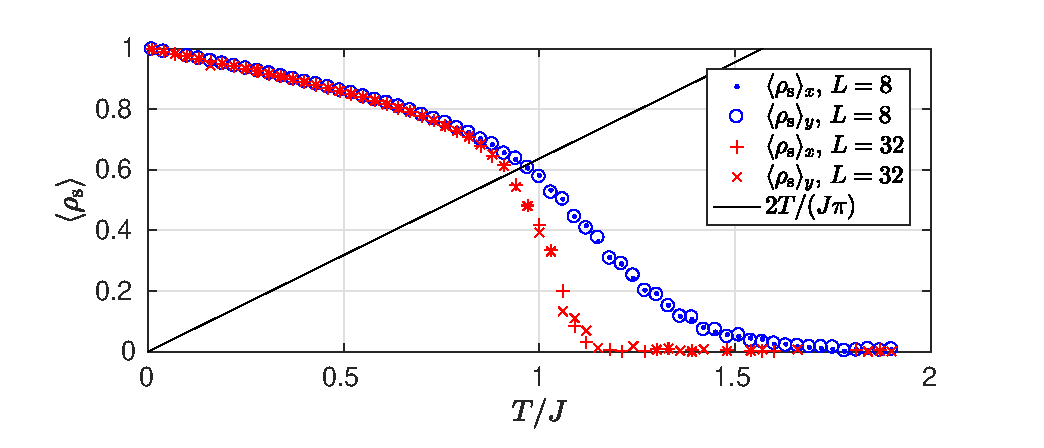
\includegraphics[width=1\textwidth]{XY_rhos_L-8-32_Nsteps-64.eps}
\caption{The spin stiffness in both the $x$ and $y$ direction plotted
  against temperature, for two $L\times L$ grids. A drop in spin
  stiffness is noticeable and much more pronounced in the $L=32$
  case. There is no appreciable difference between $\rhos$ in the two
  directions, which we would expect since the system is symmetrical
  with respect to these directions.  } 
\label{fig:rhos1}
\end{figure}


\subsubsection{Finite size scaling}
That is however only true for the specific finite size transition
temperature. To get the thermodynamic limit we use the relation
\cite{Melko-etal2004} 
\begin{equation}\label{eq:TKT(L)}
\TKT(L) = \TKT(L=\infty)\qty[1+\frac{c^2}{[\log(L/a)]^2}],
\end{equation}
where $c$ is some constant and $a=1$ is the lattice spacing. We do see
finite size effects in \figref{fig:rhos1}, with $L=32$ having a more
distinct drop in $\rhos$ than $L=8$. We also see that $\TKT(L)$ moves
down when $L$ increased.

\begin{figure}
\centering
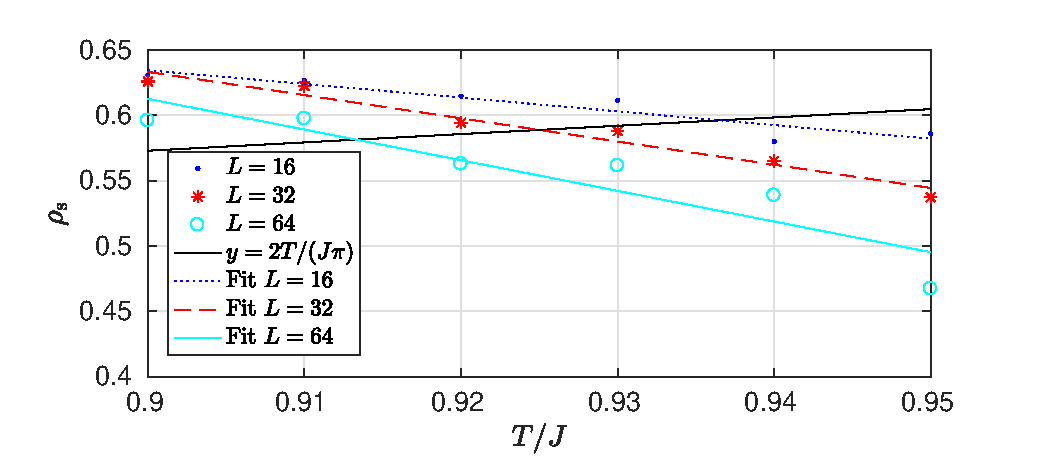
\includegraphics[width=1\textwidth]{XY_rhos_L-16--64_near-TKT.eps}
\caption{The spin stiffness $\ev{\rhos}$ and linear fits in the region
  $0.9\le T/J \le0.95$, together with the line $y=2T/(J\pi)$. The
  finite size Kosterlitz-Thouless temperatures, $\TKT(L)$, are taken to
  be the intersects between the linear fits and the line
  $y=2T/(J\pi)$. } 
\label{fig:rhos2}
\end{figure}

\begin{figure}
\centering
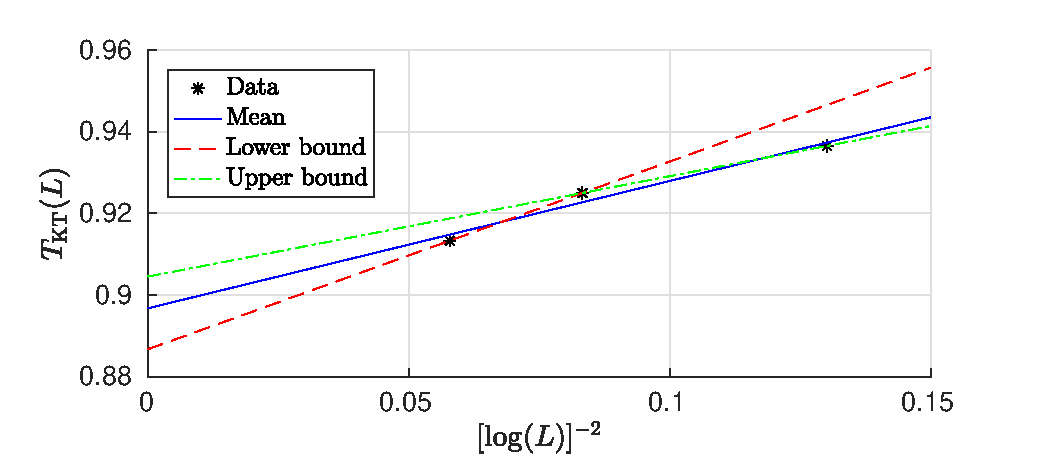
\includegraphics[width=1\textwidth]{XY_TKT_L-16--64.eps}
\caption{The $TKT$'s from \figref{fig:rhos2}, plotted against
  $[\log(L)]^{-2}$. According to \eqref{eq:TKT(L)}, the true $\TKT$
  should be where the linear fits intercepts the $y$ axis. Two more
  fits were done to get an estimate of the uncertainty of this
  estimate. } 
\label{fig:TKT}
\end{figure}

We can now perform simulations of different sized systems in the
region where we would expect the finite size Kosterlitz-Thouless
temperatures, $\TKT(L)$, to be. This is done in \figref{fig:rhos2}. 

Then we can do a linear fit on \eqref{eq:TKT(L)}, by plotting
$\TKT(L)$ against $[\log(L)]^{-2}$. The intercept of the linear fit
with the $y$ axis would then give us $\TKT=\TKT(\infty)$. From
\figref{fig:TKT}, we get the value
\begin{equation*}
\TKT = 0.897(10),
\end{equation*}
which is a bit off from the best known value of $\TKT=0.89294(8)$ but
still within the margin of uncertainty.



\subsubsection{Error sources}
There are at least two obvious error sources here. First of all, more 
simulations with more values of $L$ are needed for the fits in
\figref{fig:TKT} to be reliable. Secondly, the range
$T/J\in[0.90,0.95]$, was not suitable for the bigger systems. 

The need for more data is a constant need for anyone in science. But
in this case, I really should have done more simulations with
larger $L$'s. Three data points for a linear regression is barely what
you can call a fit. This also affects the uncertainty of the calculate
value of $\TKT$; for the error estimates, only two data points each
were used --- and that really isn't an acceptable regression.
I was however pressed on time and had to get this over with, and
this is the best I could do before I had to leave. 

Similar arguments apply to the temperature range used to find
$\TKT(L)$ in \figref{fig:rhos2}. The range should have been modified
to more even around the intersect with $y=2T/(J\pi)$. And again I will
defer back to my time situation as to why this was not mended. 

Also since, the lines in \figref{fig:rhos2} cross at so shallow
angles, the uncertainty in $\TKT(L)$ is really quite large. This
uncertainty in $\TKT(L)$ has not been regarded in the calculations of
$\TKT(L=\infty)$, which probably would have resulted in an even larger
uncertainty in the final result. 









\bibliographystyle{ieeetr}
\bibliography{ref}

\end{document}




%  LocalWords:  MFT MF Ising Ornstein Zernike Stratonovich GLW RG TKT
%  LocalWords:  rescale quartic rescaled anisotropy RNG stdlib
%  LocalWords:  Kosterlitz Thouless
